\documentclass[border={0.1cm 0.1cm 0.1cm 0.1cm}]{standalone}  %E,S,W,N

\usepackage{amssymb}
\usepackage{amsmath}
\usepackage{tikz}

\begin{document}
	
	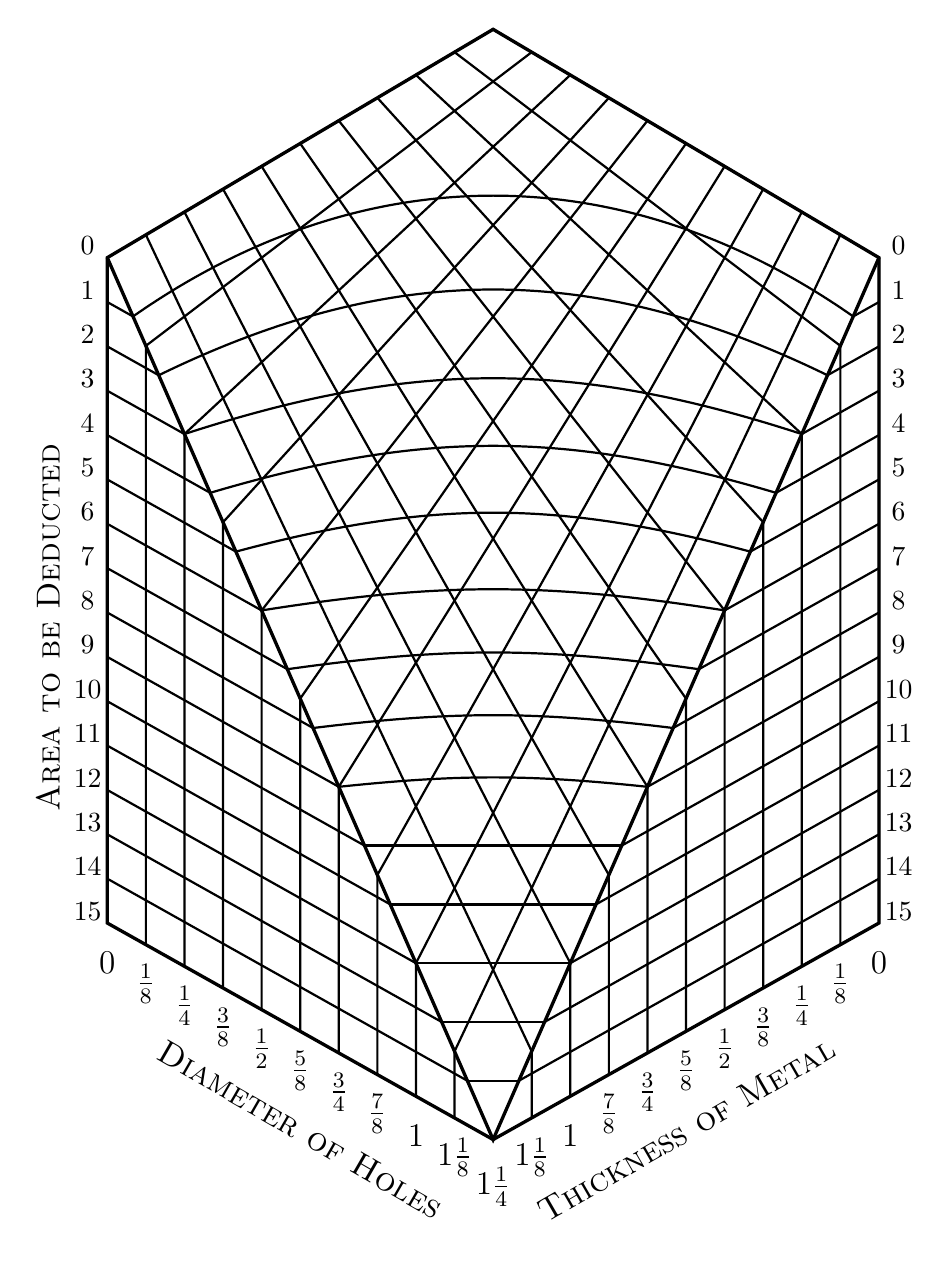
\begin{tikzpicture}[thick]
	%OUTLINE
	\draw[very thick] (0,0)--(-4.9,2.75)--(-4.9,11.2)--(0,14.1)--(4.9,11.2)--(4.9,2.75)--(0,0)--cycle;
	\draw[very thick] (-4.9,11.2)--(0,0)--(4.9,11.2);
	
	%VERTICAL LINES
	\foreach \i in {1,...,10}{
		\draw (-4.9*\i/10,2.75*\i/10)--(-4.9*\i/10,11.2*\i/10)--(4.9-4.9*\i/10,11.2+2.9*\i/10);
		\draw ( 4.9*\i/10,2.75*\i/10)--( 4.9*\i/10,11.2*\i/10)--(-4.9+4.9*\i/10,11.2+2.9*\i/10);
	}
	
	%HORIZONTAL LINES
	\foreach \i in {1,...,14}{
		\draw (-4.9,2.75+8.45*\i/15)--(-4.9*\i/15,11.2*\i/15);
	%	\draw (4.9*\i/15,11.2*\i/15) to[out={180-\i*1.5},in={0+\i*1.5}] (-4.9*\i/15,11.2*\i/15);
		\draw ( 4.9,2.75+8.45*\i/15)--( 4.9*\i/15,11.2*\i/15);
	}
	
	%CURVES -- find a more elegant formula for this
	\foreach \i in {1,...,5} \draw (4.9*\i/15,11.2*\i/15) -- (-4.9*\i/15,11.2*\i/15);
	\foreach \i in {6,...,9} \draw (4.9*\i/15,11.2*\i/15) to[out={180-\i*1},in={0+\i*1}] (-4.9*\i/15,11.2*\i/15);
	\foreach \i in {10,11,12} \draw (4.9*\i/15,11.2*\i/15) to[out={180-\i*1.5},in={0+\i*1.5}] (-4.9*\i/15,11.2*\i/15);
	\foreach \i in {13} \draw (4.9*\i/15,11.2*\i/15) to[out={180-\i*2},in={0+\i*2}] (-4.9*\i/15,11.2*\i/15);
	\foreach \i in {14} \draw (4.9*\i/15,11.2*\i/15) to[out={180-\i*2.5},in={0+\i*2.5}] (-4.9*\i/15,11.2*\i/15);
	
	%NUMBERS
	\foreach \n in {0,...,15}{
		\node at (-4.9-0.25,11.2-8.45*\n/15+0.15) {\n};
		\node at ( 4.9+0.25,11.2-8.45*\n/15+0.15) {\n};
	}
		
	%FRACTIONS -- can't use in loop because {} in frac
	\node at (-4.9+0*4.9/10,2.75-2.75*0/10-0.5) {\large 0}; 
	\node at ( 4.9-0*4.9/10,2.75-2.75*0/10-0.5) {\large 0};
	%
	\node at (-4.9+1*4.9/10,2.75-2.75*1/10-0.5) {\large $\frac{1}{8}$}; 
	\node at ( 4.9-1*4.9/10,2.75-2.75*1/10-0.5) {\large $\frac{1}{8}$};
	%
	\node at (-4.9+2*4.9/10,2.75-2.75*2/10-0.5) {\large $\frac{1}{4}$}; 
	\node at ( 4.9-2*4.9/10,2.75-2.75*2/10-0.5) {\large $\frac{1}{4}$};
	%
	\node at (-4.9+3*4.9/10,2.75-2.75*3/10-0.5) {\large $\frac{3}{8}$}; 
	\node at ( 4.9-3*4.9/10,2.75-2.75*3/10-0.5) {\large $\frac{3}{8}$};
	%
	\node at (-4.9+4*4.9/10,2.75-2.75*4/10-0.5) {\large $\frac{1}{2}$}; 
	\node at ( 4.9-4*4.9/10,2.75-2.75*4/10-0.5) {\large $\frac{1}{2}$};
	%
	\node at (-4.9+5*4.9/10,2.75-2.75*5/10-0.5) {\large $\frac{5}{8}$}; 
	\node at ( 4.9-5*4.9/10,2.75-2.75*5/10-0.5) {\large $\frac{5}{8}$};
	%
	\node at (-4.9+6*4.9/10,2.75-2.75*6/10-0.5) {\large $\frac{3}{4}$}; 
	\node at ( 4.9-6*4.9/10,2.75-2.75*6/10-0.5) {\large $\frac{3}{4}$};
	%
	\node at (-4.9+7*4.9/10,2.75-2.75*7/10-0.5) {\large $\frac{7}{8}$}; 
	\node at ( 4.9-7*4.9/10,2.75-2.75*7/10-0.5) {\large $\frac{7}{8}$};
	%
	\node at (-4.9+8*4.9/10,2.75-2.75*8/10-0.5) {\large 1};
	\node at ( 4.9-8*4.9/10,2.75-2.75*8/10-0.5) {\large 1};
	%
	\node at (-4.9+9*4.9/10,2.75-2.75*9/10-0.5) {\large $1\frac{1}{8}$}; 
	\node at ( 4.9-9*4.9/10,2.75-2.75*9/10-0.5) {\large $1\frac{1}{8}$};
	%
	\node at (0,-0.6) {\large $1\frac{1}{4}$};
	
	%LABELS
	\node at (-4.9-0.75,6.5) {\rotatebox{90}{\scshape\large Area to be Deducted}};
	\node at (-2.45,1.375-1.25) {\rotatebox{-30}{\scshape\large Diameter of Holes}};
	\node at ( 2.45,1.375-1.25) {\rotatebox{30}{\scshape\large Thickness of Metal}};
	\end{tikzpicture}
	
\end{document}